\section{Background}

Our work focuses on energy saving in cloud storage systems through the use of
block level caching mechanisms. We use DM-Cache as the block level caching
mechanism to evaluate our work on as it is freely available as a Linux kernel
module and is currently in use in many cloud storage systems such as Facebook's
FlashCache which is based on the implementation of DM-Cache \cite{flashcache}.

\subsection{Cloud Storage Systems}

Due to the physical limitation of local storage, many enterprise solutions
choose to employ Storage Area Networks, or SAN's, in an attempt to centralize
storage access and provide larger storage capabilities. SAN's also provide for
simplification of virtual machine migration and increased data reliability. Due
to the central nature of the storage this means that multiple nodes will use the
same storage node for all their data needs. For the storage node this means
satisfying multiple requests from many different machines and being able to do
so quickly. Because the storage is no longer local this increases request
latency as the storage node is further from the client and has to service
multiple clients at a time. With this kind of storage bottlenecks such as
network bandwidth and I/O throughput can play large roles in both performance
and power consumption.

\subsection{Local SSD Caching}

Usage of SSD's as primary storage is impractical because of cost and storage
size. The cost of an SSD per gigabyte is much higher than that of conventional
HDD's and their storage size is very limited compared to multi terabyte hard
disks. SSD performance is much higher than HDD's as there are no mechanical
parts which makes them ideal to use as cache devices.

Using an SSD as a local cache device diverts some read requests from the
mechanical drive to the much faster and more energy efficient SSD. The more
requests that can be satisfied using the local cache device the higher the
performance gains for the workload. This also saves energy as the requests are
now being satisfied by a more power efficient storage mechanism than standard
mechanical drives.

Figure \ref{fig:dm-cache} shows local SSD caching in practice in the cloud
environment. Multiple nodes are connected to a Storage Area Network where the
centralized storage is located. When these nodes need to access data located on
the central storage server they have to issue a request to it. Since multiple
nodes are using this storage server this means that this request may have to
wait for others to complete before it can be completed. Using a local cache
device on the client node it is possible to cache some of these requests such
that subsequent requests do not need to go to the central storage server. This
alleviates wait times on the storage server since less requests are sent to it
and reduces the time that an application has to wait for a request since the
information is now on a local cache device which has a much faster response
time.

\subsection{Disk and SSD Power Consumption}

\begin{table}[t]
  \centering
  \resizebox{\linewidth}{!}
  {
    \begin{tabular}{|l|l|l|l|l|l|}
      \hline
      \bf Disk-State & \bf Watts & \bf Inc. from Inactive & \bf Disk-State & \bf
      Watts & \bf Inc. from Inactive \\ \hline
      HDD-Inactive:       & 142.7 & +0   & SSD-Inactive:       & 130.1 & +0   \\
      \hline
      HDD-Idle:           & 146.7 & +4   & SSD-Idle:           & 130.8 & +0.7 \\
      \hline
      HDD-Active (Read):  & 149.9 & +7.2 & SSD-Active (Read):  & 133.6 & +3.5 \\
      \hline
      HDD-Active (Write): & 150.3 & +7.6 & SSD-Active (Write): & 135.2 & +5.1 \\
      \hline
    \end{tabular}
  }
  \caption{Power consumption of HDD's vs. SSD's}
  \label{tab:power-consumption}
\end{table}

We performed some simple benchmarking tests on HDD's and SSD's to get an insight
of their respective power consumption. Table ~\ref{tab:power-consumption} shows
the results for disks that we are currently using in a cluster in our lab.

\begin{table}[t]
  \centering
  \resizebox{\linewidth}{!}
  {
    \begin{tabular}{|l|l|l|l|}
      \hline
      \bf Disk-Operation & \bf Energy Consumed (J) & \bf Disk-Operation & \bf
      Energy Consumed (J) \\ \hline
      HDD-Read:  & 734.2  & SSD-Read:  & 212.5 \\ \hline
      HDD-Write: & 1127.8 & SSD-Write: & 561.2 \\ \hline
    \end{tabular}
  }
  \caption{Energy consumption of read and write operations for 12GB files}
  \label{tab:energy-consumption}
\end{table}

These results show the power consumption during a second for a specific power
state of the disk, in comparison to running the system with an inactive
drive. The power consumption during idle disk states shows that HDD's consume
more than four times the power consumption of an SSD. The reason for this is
that HDD's are constantly spinning even when not serving I/O requests, whereas
SSD's use very little power since they don't possess any mechanical parts. When
we add the additional power consumption of sequential I/O operations, reads
consume more than twice the power in comparison to SSD's.

These figures were obtained while performing write and read operations for a
12GB file. They are the average of the power consumption for each
operation. Based on these figures the energy consumed for each operation can be
seen in Table ~\ref{tab:energy-consumption}.

The results show that there's a clear advantage to using SSD's instead of HDD's
when it comes to energy savings.

\subsection{DM-Cache}

\begin{figure}[t]
  \caption{Architecture of DM-Cache}
  \centering 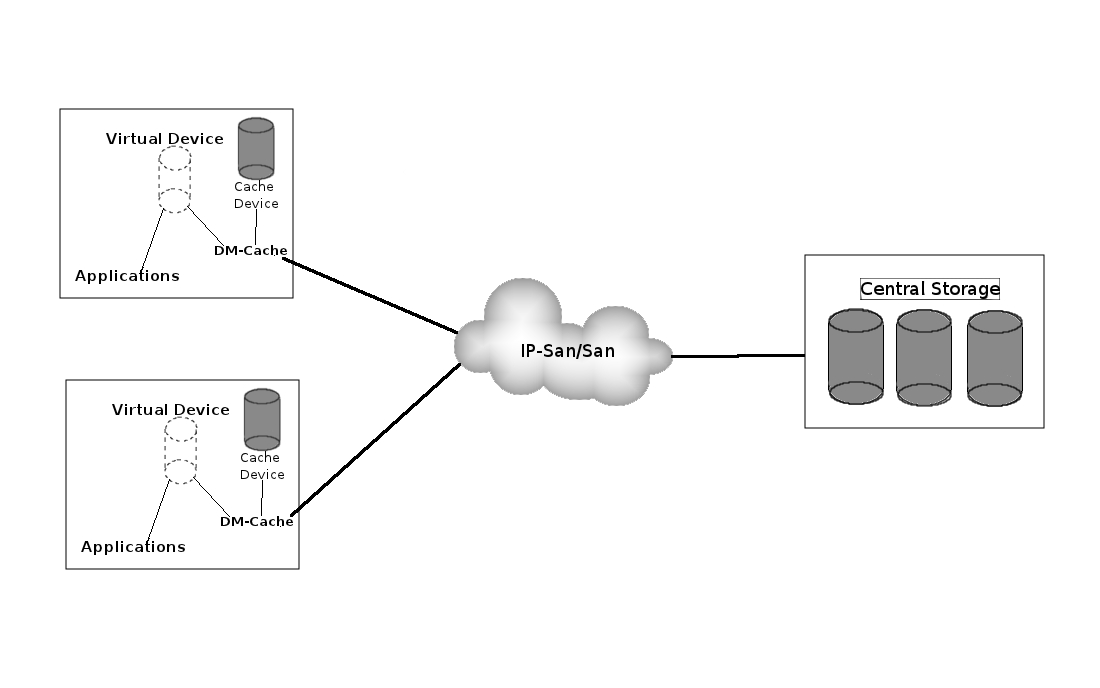
\includegraphics[width=\linewidth]{dm-cache_diagram.jpg}
  \label{fig:dm-cache}
\end{figure}

DM-Cache, or Device Mapper Cache, is a block-level caching mechanism implemented
as a module in the Linux kernel \cite{DM-Cache}. It allows for specification of
a local SSD as a cache device where recently used blocks can be stored for
faster access time. It supports both write-back and write-through functionality
for handling cached data. Figure ~\ref{fig:dm-cache} shows the architecture of
DM-Cache.

The purpose of DM-Cache is to cache recently used blocks on local storage
instead of retrieving them from some external storage source. This helps to
alleviate network bandwidth issues as well as reduce response times and save
power by issuing less requests to the storage nodes which use mechanical disks.

The current implementation of DM-Cache uses a hash table that maps logical block
addresses to entries within the hash table and evictions are done when two block
addresses map to the same entry but contain different data. This eviction scheme
does not take into account most recently used blocks and it also does not make
any attempt to pre-fetch any other blocks. Our work expands DM-Cache's cache
eviction policy to make smarter decisions in order to increase performance and
save energy.

\subsection{Effect of Spinning Down Disks}

Generally, a spun down disk consumes less power than a spinning disk. While the
spinning down of mechanical disks during idle time can reduce power consumption,
it can also be detrimental to the disks lifetime. Frequent disk spin down causes
physical damage due to the head load/unload cycles that are performed. Low
performance disks can withstand up to 500,000 spin downs in their lifetime. On
the other hand, enterprise disks, which are higher performance disks that data
centers usually use, are not intended to be spun down frequently. These disks
can only tolerate around 25,000 disk spin downs, which limits the amount of
times they may be spun down per hour. Seagate Constellation ES drives should not
be spun down more than once every 15 minutes.  The spinning down of disks also
impacts performance as it takes 6-10 seconds to spin up a disk after it has been
spun down.
